% Number 600
% CAPMA CAPMG Algebra Units 
% Overtaking - CAPM and CVPM
% JG

% Watermark
\AddToShipoutPicture*{\BackgroundPic}

\addtocounter {ProbNum} {1}

%\begin{floatingfigure}[r]{.2\textwidth}
%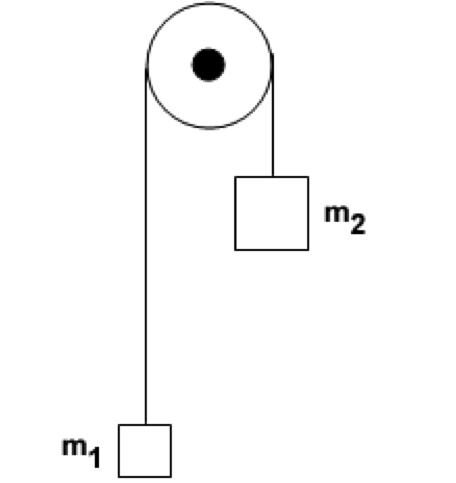
\includegraphics[scale=.8]{/Users/jgates/desktop/latex/pics/Atwood3}
%\end{floatingfigure}
 
{\bf \Large{\arabic{ProbNum}}} A police car is driving towards a parked pair of criminals eating Zagnuts after pulling off a heist. The police car is moving ${40~\tfrac{m}{s}}$ and is initially .4 km away from the criminals. The criminals are going to drive away from the police car in an attempt to escape.  Assume that the crimemobile moves with a constant acceleration of ${1.8~\tfrac{m}{s^2}}$. 

\bigskip
Where will the police catch them?

\vfill

Draw a velocity graph for the criminals.  Use it to determine how far down they road they are when the police car passes their starting point.
\vfill

%\hfill 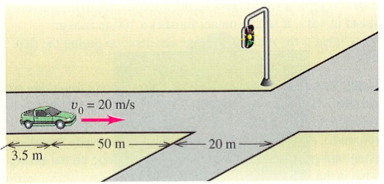
\includegraphics[scale=.85]{/Users/jgates/desktop/latex/pics/redlight.png}
\newpage